\section{Introducción a Apolo y mejoras en el 2013}

\subsection{¿Qué es Apolo?}
Apolo, el Centro de Computación Científica ubicado en la Universidad EAFIT en Medellín, Colombia, tiene por objetivo principal apoyar investigaciones, así como a las diferentes industrias en la aceleración de los tiempos de ejecución de simulaciones computacionales utilizando técnicas de computación de alto rendimiento, también conocida como computación paralela. Para esto cuenta con un equipo humano capacitado y un clúster computacional que permite ejecutar programas de manera paralela, de forma tal que procesos que podrían tomar meses o incluso años ejecutándose se podrían reducir a semanas u horas. Es por ello que Apolo se vuelve un recurso estratégico, no sólo para la Universidad sino para la nación, apoyando la investigación y el desarrollo del país y de la región. 

\subsection{Mejoras en la infraestructura lógica y de servidores}

Apolo inició actividades en 2012 con la donación de 40 servidores con 4 núcleos realizada por la Universidad Purdue, de Estados Unidos. A partir de ese momento son varias las mejoras y adiciones que se han realizado al centro de cómputo. Dentro de ellas se encuentra la integración a Apolo de un cluster, ya existente en EAFIT, perteneciente al grupo de Investigación en Mecánica Aplicada, agregando así 6 servidores más, quedando un total de 46 servidores y 208 núcleos de cómputo en el año 2012, dedicados completamente al servicio de la investigación tanto para EAFIT como para otras universidades de la ciudad.
En 2013 el Centro de Informática y la Dirección de Investigación de la Universidad, decidieron continuar el convenio con la Universidad Purdue y comprar 40 nodos más, esta vez, los servidores son de 8 núcleos, teniendo entonces el centro de cómputo 86 servidores y un total de 528 núcleos. Uno de los avances más importantes que se hizo en la infraestructura lógica de Apolo fue el diseño, instalación y puesta en marcha de un sistema de colas, que permite a los administradores del sistema controlar mucho mejor los trabajos lanzados por los usuarios y además posibilita llevar estadísticas de uso mucho más detalladas. Desde la perspectiva del usuario será mucho más fácil garantizar que sus trabajos se están corriendo de manera correcta y con el mejor rendimiento posible, reservando máquinas para solo sus propias simulaciones sin interferir con las de otros científicos. Este sistema se instaló en el mes de agosto. 

\begin{figure}[ht]
  \centering
  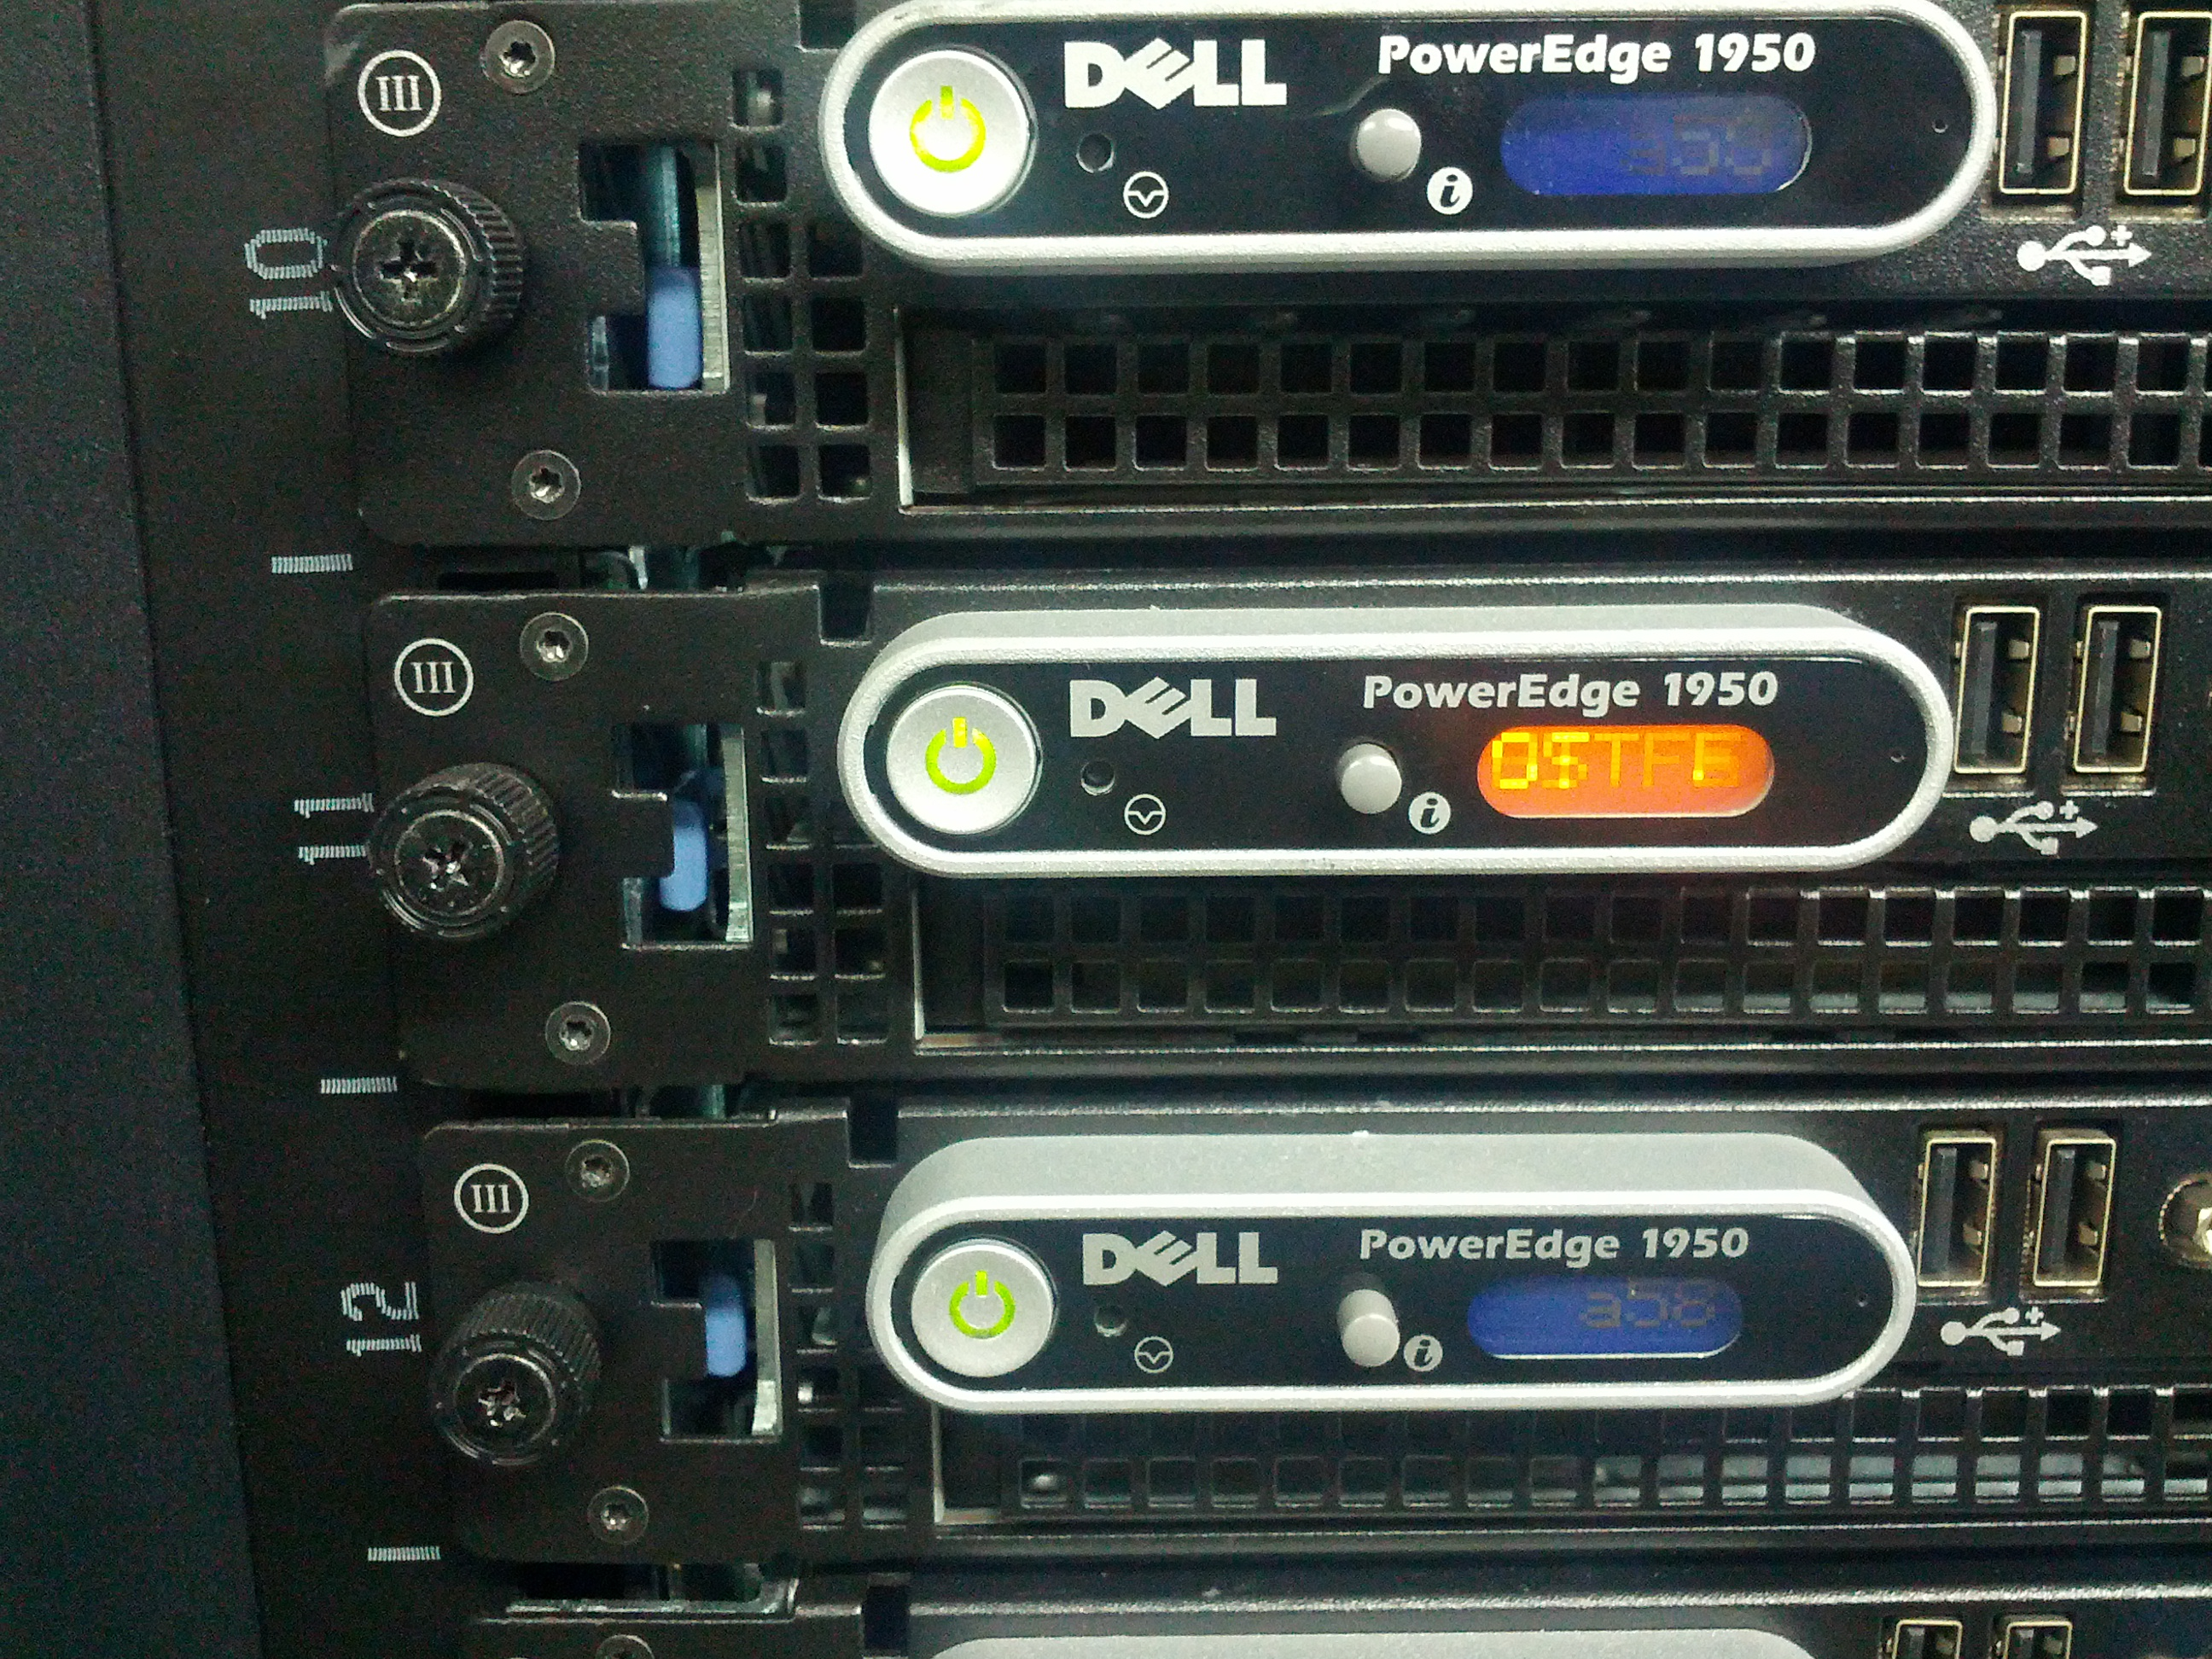
\includegraphics[scale=0.15]{imgs/dell.jpg}
  \caption{Servidores DELL 1950 de 8 núcleos.}
  \label{fig:dell}
\end{figure}

%Apolo inició actividades en el año 2012 a partir de la donación de 40 servidores con 4 núcleos, dicha donación fué realizada por la Universidad Purdue. A partir de ese momento son varias las mejoras y adiciones que se han hecho al centro de cómputo. Posteriormente a Apolo se adicionó un cluster ya existente en EAFIT, perteneciente al grupo de Investigación en Mecánica Aplicada, agregando así 6 servidores más, quedando un total de 46 servidores y 208 núcleos de cómputo en el año 2012 dedicados completamente al servicio de la investigación tanto para EAFIT como para otras universidades de la ciudad. En el año 2013 el Centro de Informática y la Dirección de Investigación decidieron seguir el convenio con la Universidad Purdue y comprar 40 nodos más, esta vez, los servidores son de 8 núcleos, quedando así el céntro de cómputo con 86 servidores y un total de 528 núcleos.

%Actualmente Apolo es un clúster de servidores híbrido, ya que cuenta con tres tipos de servidores distintos, los cuales se dividen de la siguiente manera: 40 Servidores Dell de 8 nucleos , 40 Servidores HP de 4 nucleos, 6 Servidores Blade HP de 8 nucleos,  para un total de 86 Maquinas y 528 Nucleos. Con un TB de memoria RAM distribuida, todo sobre arquitectura Intel de 64 bits y soportado en el sistema operativo Linux. También cuenta con una red Ethernet interna de 1 GBps.


\subsection{Mejoras en la infraestructura física}
En el transcurso del año 2013 se hicieron varias mejoras al centro de datos que contiene el clúster computacional. Las mejoras principales son las siguientes:
\begin{itemize}
\item \textbf{Diseño eléctrico:} Se adaptó el tablero eléctrico para soportar las nuevas 40 máquinas provenientes de la Universidad Purdue.
\item \textbf{Piso falso:} Dado el recalentamiento de algunos de los servidores se realizó el diseño y la implementación de un piso falso con la ayuda del Grupo de Investigación en Mecánica Aplicada y Servicios Generales. Este piso ayuda a garantizar que los servidores tienen una temperatura adecuada para el correcto funcionamiento en el proceso de computación.
\item \textbf{UPS:} Se adicionaron dos módulos de UPS a la infraestructura para soportar los servidores adicionales y darle tiempo adicional de autonomía al centro de datos en caso de falla eléctrica.
\end{itemize}

\subsection{Equipo humano}

Apolo cuenta con un coordinador científico, un coordinador técnico, cuatro estudiantes de pregrado como auxiliares de administración, un estudiante de maestría realizando su tesis en computación de alto rendimiento y un estudiante de pregrado con su proyecto final de grado enfocado en el uso de computación de alto rendimiento. Este año se enviaron cuatro de los estudiantes de pregrado que trabajan en Apolo al programa S.U.R.F en la Universidad Purdue, éste es un programa de verano en el cual los estudiantes reciben entrenamiento en distintos temas de investigación, colaboran desde sus áreas de estudio en varios desarrollos y tienen la oportunidad de trabajar en laboratorios de investigación, algunos de estos en temas de computación de alto rendimiento. Desde esta experiencia, cada uno de los estudiantes participó en el desarrollo herramientas para distintas plataformas de computación de alto rendimiento, entre ellas \textit{nanohub}\footnote{http://www.nanohub.org}, dando como resultado la coautoría en varios artículos publicados por la Universidad Purdue.

Este año también el centro de computación empezó a trabajar con estudiantes becados del Fondo EPM, pensando en la multidisciplinariedad ingresó un estudiante de segundo semestre de Economía para ayudar con labores básicas.

\begin{figure}[ht]
  \centering
  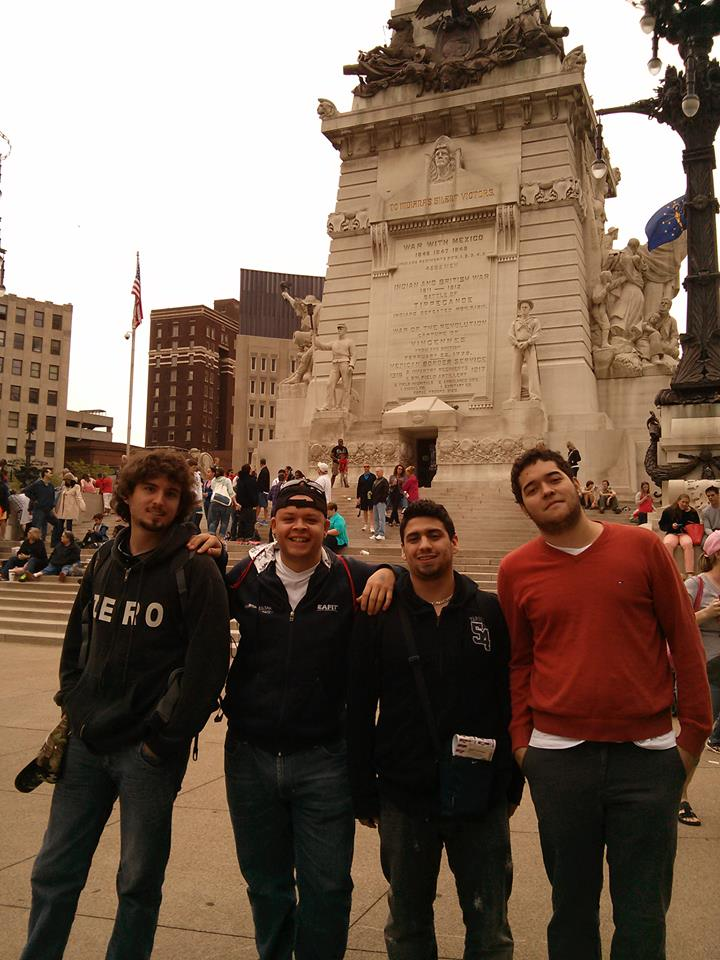
\includegraphics[scale=0.3]{imgs/loscuatro2.jpg}
  \caption{Estudiantes de Pregrado que trabajan en Apolo.}
  \label{fig:guys}
\end{figure}


\section{Uso de Apolo durante 2013}
2013 fue un año especial para Apolo, ya que comenzó a ser visible en el país y así se evidenció en el Segundo Encuentro Internacional de E--Ciencia, en la ciudad de Santiago de Cali, donde hubo la oportunidad de interactuar con otras universidades y homólogos de clusters computacionales de Colombia, como Guane--1 de la Universidad Industrial de Santander y BIOS del Centro de Bioinformática y Biología Computacional. Otro aspecto importante es que Apolo también se dió a conocer no solo en contexto académico sino también en el industrial, así lo demuestra el contacto que se tuvo con algunas compañías que requieren computación de alto rendimiento para sus productos, como INDISA S.A. y Tezio S.A.S.


Algunos datos acerca del uso de Apolo se muestran a continuación.

\subsection{Grupos de investigación y publicaciones}
A lo largo del semestre el Centro de computación Apolo:

\begin{itemize}
\item Ayudó con recursos y capacitaciones de computación de alto rendimiento a 12 grupos de investigación de la Universidad EAFIT
\item Colaboró con capacidad de cómputo a 3 Universidades Colombianas y una Universidad Argentina
\item Ayudó en la producción de 13 publicaciones en revistas de investigación y una tesis de maestría
\item Colabora con las simulaciones de 23 investigadores, 8 estudiantes de doctorado, 22 estudiantes de maestría, 3 estudiantes de pregrado
\end{itemize}

\subsection{Estadísticas de uso}

\subsubsection{Sistema de colas}

Desde la puesta de funcionamiento del sistema de contabilidad y colas desde el 3 de agosto hasta el 12 noviembre de 2013 se tienen las siguientes estadísticas:

\begin{itemize}
\item Se han ejecutado un total de 9154 simulaciones
\item En total se han ejecutado 119813 horas, el equivalente a 13.67 años durante 3 meses y medio.
\item Los grupos que más han usado Apolo son:
  \begin{itemize}
    \item Ingeniería Física
    \item Ingeniería Mecánica
    \item Economía
  \end{itemize}
\end{itemize}


\section{Benchmark Lartop 50}

En el presente año, el Centro de Computación Científica APOLO fue invitado a participar en el \textit{ranking} de las 50 Supercomputadoras más rápidas en Latinoamérica, obteniendo el lugar número 11 con 1 TeraFLOPS\footnote{\textbf{FLOPS:} Float point Operation Per Second} demostrado. Este \textit{benchmark} se realizó con LinPACK, software proporcionado por el \textit{ranking} mundial de supercomputadoras Top500\footnote{http://www.top500.org}.

\section{Nanohub}
Actualmente se continúa con el desarrollo del espejo del nanohub con la Universidad Purdue. Este año se realizó la interconexión entre dicha infraestructura y Apolo, logrando que Apolo se viera como un lugar más de cómputo para simulaciones realizadas en Purdue.

\section{Hub de Ciencia Regional}
Como iniciativa en conjunto con el grupo de Investigación Research In Spatial Economics (RiSE), se ha iniciado el diseño, desarrollo y puesta en marcha del hub de ciencia regional, el cual apunta a ser uno de los puntos de encuentro y colaboración científica a nivel mundial en esta área de la ciencia. Actualmente se encuentra en fuerte desarrollo y ya se tienen algunas simulaciones funcionando en esta herramienta gracias a la capacitación que los estudiantes, que trabajan en Apolo, recibierion en el S.U.R.F. en la Universidad Purdue.


\section{World Community Grid}

En el mes de agosto finalizó la ejecución de una simulación para la Búsqueda de una droga para la Leishmaniasis, proyecto para el cual Apolo donaba su tiempo libre. Este proyecto pertenece al Programa de Estudio y Control de Enfermedades Tropicales (PECET) de la Universidad de Antioquia y se computaba por medio del World Community Grid, una infraestructura de cómputo que permite a individuos e instituciones aprovechar sus recursos computacionales, donando tiempo de ejecución cuando estos no son utilizados. Una vez terminada esta simulación se procedió a dedicar el tiempo libre del clúster de Apolo a la lucha contra el VIH con el proyecto FightAIDS@HOME, inscrito también World Community Grid.


Algunos datos interesantes de Apolo con respecto al World Community Grid son:

\begin{itemize}
\item Desde su comienzo en febrero de 2012, Apolo a donado el equivalente a 152 años de cómputo al World Community Grid.
\item En el proyecto de ``Drug Search for Leishmaniasis'' Apolo aportó aproximadamente 104 años de cómputo
\item En el proyecto de ``FightAIDS@HOME'' Apolo hasta ahora ha realizado calculos equivalentes a 48 años
\item Apolo está en la posición 278 de más de 600.000 usuarios que colaboran con el World Community Grid.
\end{itemize}

\section{Comportamiento de Apolo durante el año}
En este apartado se analizará el comportamiento e incidentes que se tuvieron durante el año y como se ven estos reflejados en las estadísticas de uso de Apolo.

\subsection{Carga}
\begin{figure}[ht]
  \centering
  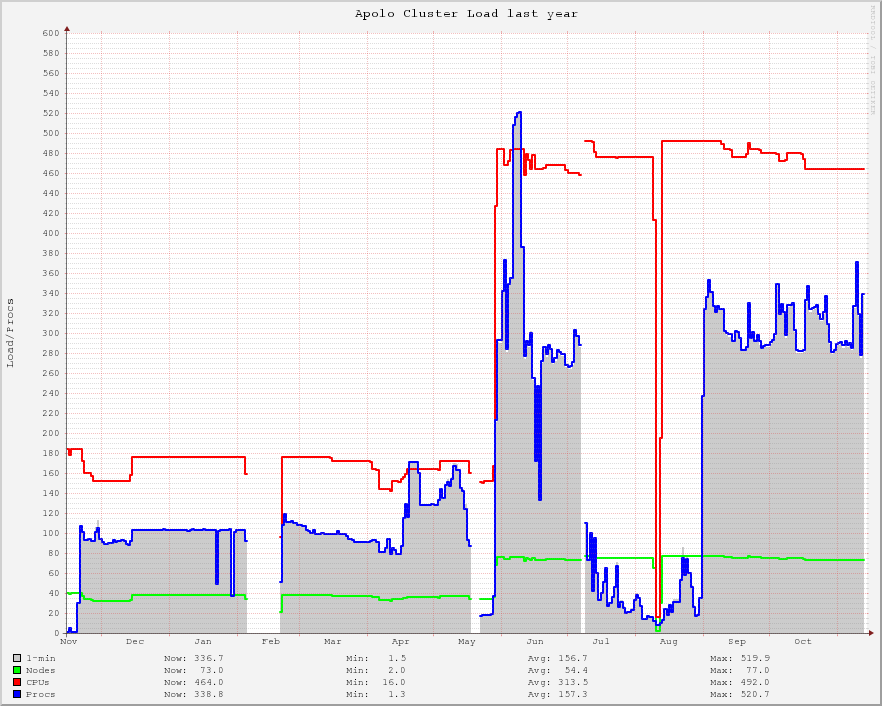
\includegraphics[scale=0.45]{imgs/load2013.png}
  \caption{Carga de Apolo durante 2013.}
  \label{fig:load}
\end{figure}

Como se puede observar en la figura \ref{fig:load}, la carga de Apolo tuvo algunas interrupciones a lo largo del año, existen algunos vacíos al principio de febrero debido a problemas con el aire acondicionado e incidentes en la parte eléctrica del datacenter. A mediados de mayo vemos otra caida en la carga útil de Apolo, la cual refleja la puesta en marcha de los 40 módulos nuevos que se trajeron desde la Universidad Purdue y mejoras eléctricas en el centro de datos. Finalmente vemos una pequeña baja principios de Julio la cual fue necesaria para la puesta en marcha del nuevo sistema de colas. Las líneas verde y roja representan el número de núcleos y el número de CPU's en Apolo, respectivamente, las cuales no se mantienen constantes debido a fallas fortuitas en algunos módulos de memoria y discos debido al uso intensivo que estos han tenido. Igualmente se puede notar el aumento considerable en el número de núcleos y CPU's\footnote{Las primeras máquinas de Apolo tienen 2 CPU's y 4 núcleos, mientras que las que se agregaron este año son de 2 CPU'S y 8 núcleos.} en Apolo, ya que como se visualiza con las líneas roja y verde, se agregaron al clúster 320 núcleos o 80 CPU's de 8 núcleos. El número de procesos lanzados en Apolo incrementa considerablemente a finales de agosto y se mantiene durante los meses de septiembre, octubre y noviembre hasta la fecha. Un hecho notable es el pico de carga que se observa a inicios de junio, justo en el momento de la realización del \textit{benchmark} para enviar al top de las 50 supercomputadoras más rápidas de Latinoamérica LarTOP50, el cual demuestra que Apolo estaba siendo consumido en su totalidad por parte de dicho \textit{benchmark}.

\subsection{Memoria}
\begin{figure}[ht]
  \centering
  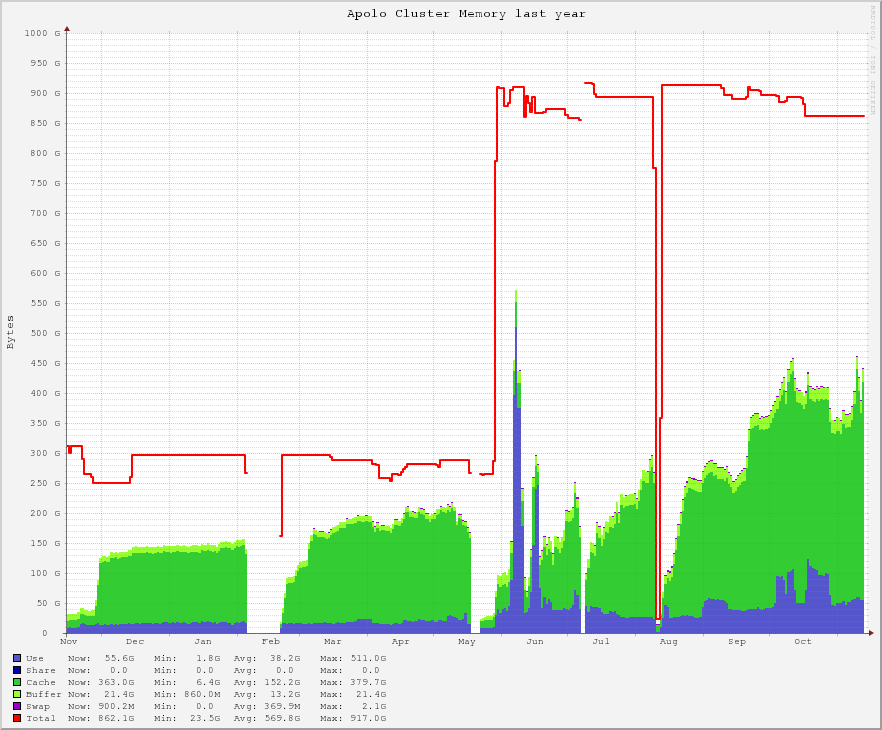
\includegraphics[scale=0.45]{imgs/memory2013.png}
  \caption{Memoria de Apolo durante 2013.}
  \label{fig:mem}
\end{figure}

En la figura número \ref{fig:mem} se visualiza la cantidad de memoria utilizada a lo largo del año por los distintos procesos lanzados en Apolo, es notorio que con la actualización y las máquinas adicionales las simulaciones en Apolo no consumen toda la cantidad disponible de memoria de Apolo, solo al final del año se nota un aumento considerable en el consumo de memoria, los cuales están muy por debajo de los límites actuales de Apolo. Esto está relacionado con el tipo de implementación que tienen las simulaciones de los científicos y usuarios de Apolo. Al igual que en la gráfica anterior, es notorio los momentos fuera de servicio que tuvo el clúster a lo largo del año.

\subsection{CPU}
\begin{figure}[ht]
  \centering
  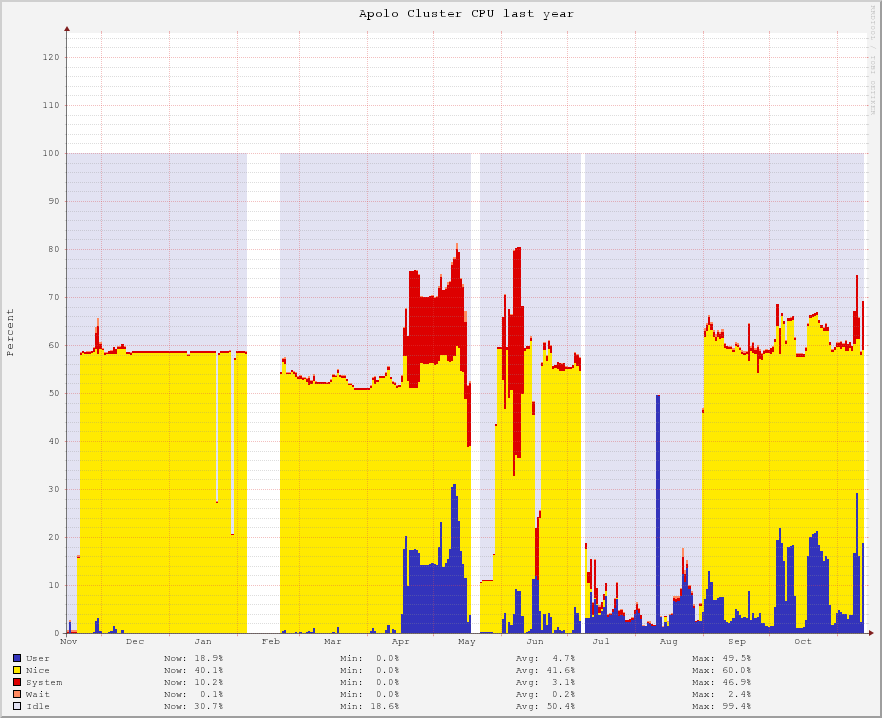
\includegraphics[scale=0.45]{imgs/cpu2013.png}
  \caption{CPU de Apolo durante 2013.}
  \label{fig:cpu}
\end{figure}

En el consumo de CPU que se muestra en la figura numero \ref{fig:cpu} a pesar de notarse consumos importantes en procesos de usuario (azul) y de sistema (rojo), aún siguen predominando los procesos de baja prioridad (amarillo), éstos últimos son en su mayoría los procesos asociados al World Community Grid. Existe un vacío importante entre los meses de julio y agosto en este último tipo de procesos, justo cuando el proyecto de ``Drug Search for Leishmaniasis'' finaliza y no es sino hasta que se decide colaborar con el proyecto ``FightAIDS@HOME'' que se retoman este tipo de procesos en Apolo.

\subsection{Red}
\begin{figure}[ht]
  \centering
  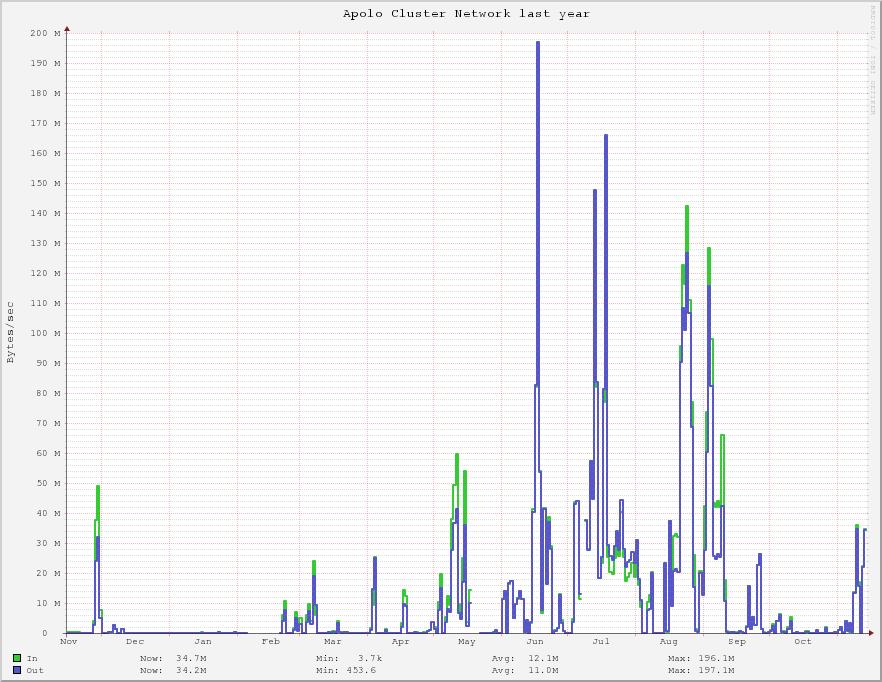
\includegraphics[scale=0.45]{imgs/network2013.png}
  \caption{Red de Apolo durante 2013.}
  \label{fig:net}
\end{figure}

Finalmente, en la figura \ref{fig:net} se observa el uso de la red el cual es notable durante el \textit{benchmark} en junio y se continua usando intermitentemente durante el resto del año. El uso de la red también depende de la naturalez y la manera que haya sido desarrollada la aplicación que se ha lanzado en Apolo.

\newpage
\section{Software Instalado}

A lo largo del año se realizarion los esfuerzos necesarios para cumplir con los requisitos de los usuarios de Apolo en cuanto al software que se requiere para hacer las simulación. A continuación se muestra una lista del software científico disponible en Apolo.

% Table generated by Excel2LaTeX from sheet 'Sheet1'
\begin{table}[htbp]
  \centering
  \caption{Software disponible en Apolo}
    \scalebox{0.8}{
    \begin{tabular}{rcr}
      \hline
    \multicolumn{1}{c}{\textbf{Software}} & \textbf{Versions in APOLO} & \multicolumn{1}{c}{\textbf{License Type}} \\
    \hline
%    \midrule
    Lammps & lammps 30/09/13 & Open Source \\
    Gurobi & 5.6.0 & Commercial \\
    BOINC & -     & Open Source \\
    Code Saturne & 3.0.1 & Open Source \\
    ESPResSo & 5.0.1 & Open Source \\
    OpenFOAM & 2.1.1 & Open Source \\
    GAMESS & -     & Open Source \\
    Crystal & 1.0.1 & Commercial \\
    Octave & 3.4.3 & Open Source \\
    ABINIT & 7.2.1 - 7.4.1 & Open Source \\
    GCC   & 4.4.6 & Open Source \\
    Python & 2.7.2 & Open Source \\
    gfortran & 4.4.6 & Open Source \\
    Paraview &  3.12     & Open Source \\
    Ansys & 14,5  & Commercial License \\
    Atlas & 3.8.4 & Open Source \\
    Cmake & 2.8.4 & Open Source \\
    FFTW2 & 2.1.5 & Open Source \\
    Git   & 1.7.1 & Open Source \\
    Glib 2 & 2.22.5 & Open Source \\
    GTK 2 & 2.18.9 & Open Source \\
    HDF5  & 1.8.5 &  \\
    Jasper & 1.900.1 & Open Source \\
    JAVA  & 6.0.  & Open Source \\
    LIbPNG & 1.2.49 & Open Source \\
    LibTool & 2.2.6 & Open Source \\
    R     & 2.15.1 & Open Source \\
    Subversion & 1.6.11 & Open Source \\
    Swig  & 1.3.40 & Open Source \\
    \multicolumn{3}{c}{BIO ROLL} \\
    HMMER & 3.0.  & Open Source \\
    NCBI BLAST & 6,1   & Open Source \\
    MpiBLAST & 1.6.0 & Open Source \\
    biopython & 1,57  & Open Source \\
    ClustalW & 2,1   & Open Source \\
    MrBayes & 3.1.2 & Open Source \\
    T\_Coffee & 8,99  & Open Source \\
    Emboss &       & Open Source \\
    Phylip & 3,69  & Open Source \\
    FASTA & 36.3.5a & Open Source \\
    Glimmer & 3,02  & Open Source \\
    TIGR Assembler & 2     & Open Source \\
    \multicolumn{3}{c}{HPC ROLL} \\
    IOzone & 3,397 & Open Source \\
    Iperf & 2.0.5 & Open Source \\
    MPICH2 & 1.4.1 & Open Source \\
    Open MPI & 1.5.3 - 1.4.3(rocks) & Open Source \\
    Stream & 5,9   & Open Source \\
    \multicolumn{3}{c}{SISTEMAS DE COLAS} \\
    Condor & 6.0.  & Open Source \\
    Torque & 4.2.3     & Open Source \\
%    \bottomrule
    \hline
    \end{tabular}%
    }
  \label{tab:addlabel}%
\end{table}%




\newpage
\section{Agradecimientos}
El Centro de Computación Apolo desea agradecer a las distintas áreas, grupos de investigación y dependencias de la Universidad que de una u otra manera hicieron posible el mantenimiento y el servicio de Apolo durante 2013. También agradece a la Universidad Purdue por el constante e incondicional apoyo que han prestado al personal de Apolo.


%% Purdue
%% Grupos de Investigación
%% Servicios Generales
